% DO NOT COMPILE THIS FILE DIRECTLY!
% This is included by the other .tex files.

\begin{frame}[t,plain]
\titlepage
\end{frame}

\begin{frame}
    \frametitle{Outline of the presentation}
    \begin{itemize}
        \item Present the features available for Sharing \textit{galaxy clusters}
        \item Look at the internals of what changed in the datamodel and MISP's behaviors
    \end{itemize}
\end{frame}

\begin{frame}
    \frametitle{MISP Galaxy 2.0}
    Galaxy 2.0 introduces various new features for \textit{Galaxies} and their \textit{Clusters} allowing:
    \begin{itemize}
        \item Creation of \textbf{custom} \textit{Clusters}
        \item ACL on \textit{Clusters}
        \item \textbf{Connection} of \textit{Clusters} via \textit{Relations}
        \item \textbf{Synchronization} to connected instances.
        \item \textbf{Visualization} of forks and relationships
    \end{itemize}
\end{frame}


\begin{frame}
    \frametitle{MISP Galaxy 2.0 - New \textit{Cluster} fields}
    \textit{Clusters} and \textit{Relations} can be edited.
    \begin{itemize}
        \item New \textit{Clusters} fields
        \item \texttt{distribution}, \texttt{sharing\_group\_id}
        \item \texttt{org\_id}, \texttt{orgc\_id}
        \item \texttt{locked}, \texttt{published}, \texttt{deleted}
        \item \texttt{default}
        \begin{itemize}
            \item \textit{Clusters} coming from the \texttt{misp-galaxies} repository are marked as default
            \item Not synchronized
        \end{itemize}
        \begin{itemize}
            \item Same purpose as \textit{Events}s \texttt{locked}
        \end{itemize}
        \item \texttt{extends\_uuid}
        \begin{itemize}
            \item Point to the \textit{Cluster} that has been forked
        \end{itemize}
        \item \texttt{extends\_version}
        \begin{itemize}
            \item Keep track of the \textit{Cluster} version that has been forked
        \end{itemize}
    \end{itemize}
\end{frame}

\begin{frame}
    \frametitle{MISP Galaxy 2.0 - Others changes}
    \begin{itemize}
        \item \textit{Role} \texttt{perm\_galaxy\_editor}
        \item Relations also have a \texttt{distribution} and can have \textit{Tags}
        \item Servers have 2 new flags
        \begin{itemize}
            \item \texttt{pull\_galaxy\_clusters}
            \item \texttt{push\_galaxy\_clusters}
        \end{itemize}
        \item Clusters \texttt{blocklist}
    \end{itemize}
\end{frame}

\begin{frame}
    \frametitle{Features in depth: CRUD}
    \begin{itemize}
        \item Standard CRUD
        \item Soft and Hard deletion
        \item Publishing
        \item Update forked cluster to keep it synchronized with its parent
        \item ACL on the \textit{Cluster} itself, not on its tag
        \begin{itemize}
            \item \texttt{misp-galaxy:{\color{blue} galaxy-type}="{\color{red} cluster UUID}"}
            \item \texttt{\tiny misp-galaxy:{\color{blue} mitre-attack-pattern}="{\color{red} e4932f21-4867-4de6-849a-1b11e48e2682}"}
        \end{itemize}
    \end{itemize}
\end{frame}

\begin{frame}
    \frametitle{Features in depth: Visualization}
    Tree view of forked Clusters 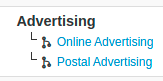
\includegraphics[scale=0.5]{pics/cluster-forks}


    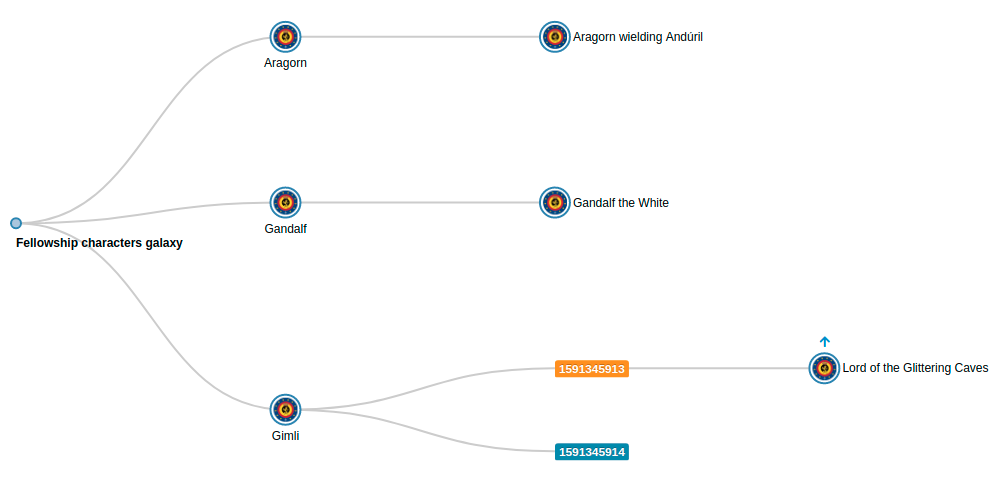
\includegraphics[width=1.0\linewidth]{pics/cluster-forks-tree}
\end{frame}

\begin{frame}
    \frametitle{Features in depth: Visualization}
    Tree and network views for Relations between Clusters
    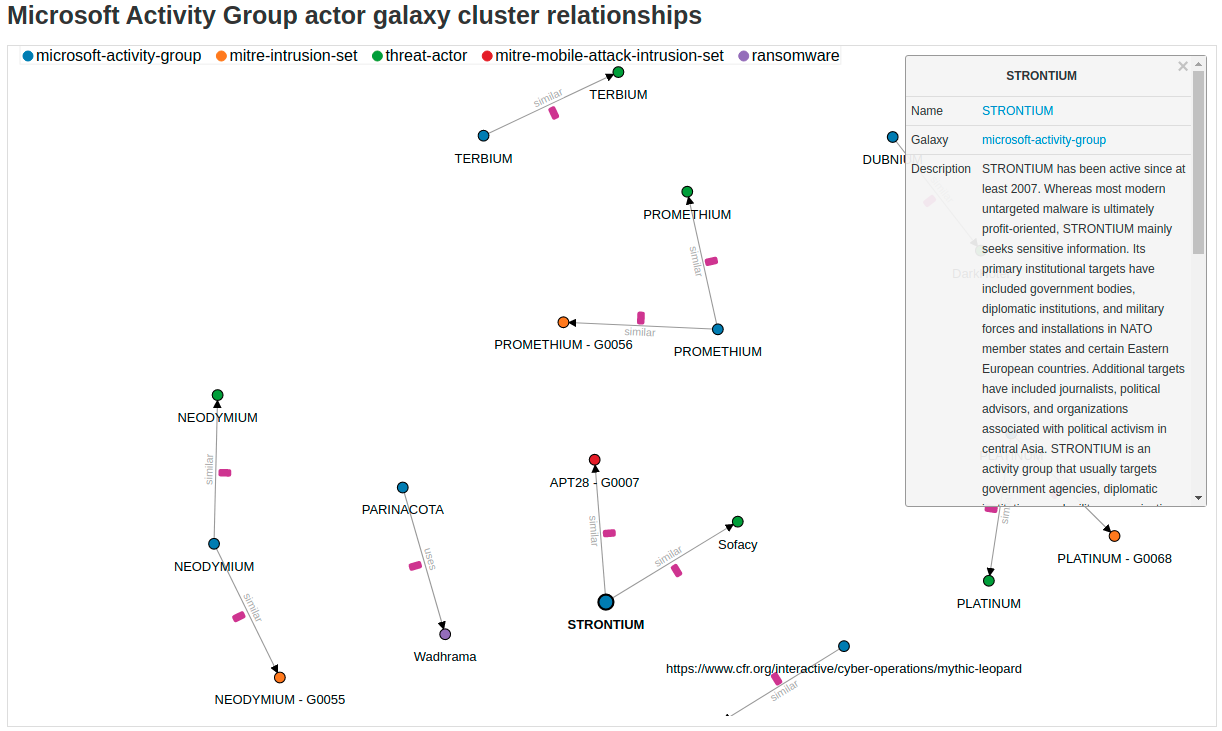
\includegraphics[width=1.0\linewidth]{pics/cluster-relations}
\end{frame}

\begin{frame}
    \frametitle{Features in depth: Visualization}
    Tree and network views for Relations between Clusters
    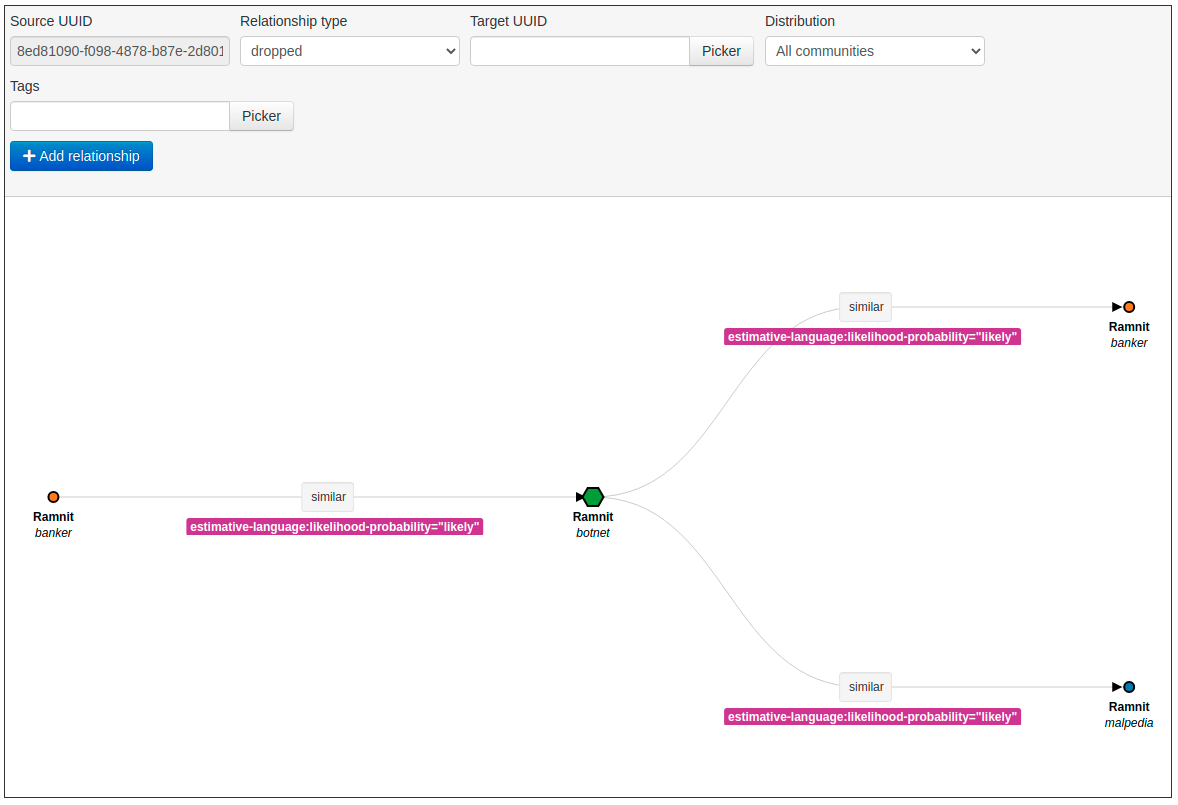
\includegraphics[width=1.0\linewidth]{pics/cluster-relations-tree}
\end{frame}

\begin{frame}
    \frametitle{Features in depth: Synchronization}
    Own synchronization mechanism which can be enabled with the \texttt{pull\_galaxy\_cluster} and \texttt{push\_galaxy\_cluster} flags

    \begin{itemize}
        \item \textbf{Pull All}: Pull all remote Clusters (similar to event's pull all)
        \item \textbf{Pull Update}: Update local Clusters (similar to event's pull update)
        \item \textbf{Pull Relevant}: Pull missing Clusters based on local Tags
        \item \textbf{Push}: Triggered whenever a Cluster is published or via standard push
    \end{itemize}
\end{frame}

\begin{frame}
    \frametitle{New views factories \& elements}
    \begin{itemize}
        \item\texttt{GenericForm.simpleFieldAllowedList}
        \begin{itemize}
            \item \texttt{checked}, \texttt{multiple}, \texttt{selected}, \texttt{legend}, \texttt{disabled},
        \end{itemize}
        \item\texttt{IndexTable.booleanOrNA}
        \begin{itemize}
            \item Displays icons or N/A
        \end{itemize}
        \item\texttt{IndexTable.galaxy\_cluster\_link}
        \begin{itemize}
            \item Display basic galaxy cluster info in a compact way (\texttt{galaxy\_type :: cluster\_value} + Hover)
        \end{itemize}
        \item\texttt{IndexTable.in\_and\_out\_counts}
        \begin{itemize}
            \item Display \# of outbound and \# of inbound (This \textit{Cluster} has \# relations)
        \end{itemize}
        \item\texttt{IndexTable.tree}
        \begin{itemize}
            \item Generate a tree like hierarchy (Root cluster and its forks)
        \end{itemize}
    \end{itemize}
\end{frame}

\begin{frame}
    \frametitle{Synchronization edge cases}
    \begin{itemize}
        \item Missing galaxy on the remote end
        \begin{itemize}
            \item[$\rightarrow$] Capture it
        \end{itemize}
    \end{itemize}
\end{frame}

\begin{frame}
    \frametitle{Impossible due to design}
    \begin{itemize}
        \item Share \textit{Galaxy Matrix}
        \begin{itemize}
            \item[$\rightarrow$] Can only be insterted in an existing \textit{galaxy} matrix as the layout is defined at the \textit{galaxy} level
        \end{itemize}
    \end{itemize}
\end{frame}
